%% in diesem Kapital steht es die Ergebnisse
\chapter{Empirische Ergebnisse} \label{Kapital4empirischeErgebnisse}
%%=======================================
\section{Die deskriptiven Ergebnisse zu den Online Consumer Reviews}
%%=======================================
Vor dem Test der Hypothesen, soll man über die ganzen Daten eine allgemeine Übersicht haben. In diesem Abschnitt werden die Wortwolken, Worthäufigkeiten und die Zeiträume von den chinesischen sowie deutschen \ac{OCRs} gebeten, um die Datenssturkturen besser zu verstehen. 

Eine Wortwolken ist eine Methode zur Informationsvisualisierung, bei der eine Liste aus Schlagworten, oft alphabetisch sortiert, flächig angezeigt wird, wobei einzelne unterschiedlich gewichtete Wörter größer oder auf andere Weise hervorgehoben dargestellt werden \citep{bateman2008seeing}. Die Abbildung \ref{fig:wortwolke} zeigt die Wortwolken von chinesischen sowie deutschen \ac{OCRs}.
\begin{figure}[h]
    \minipage{0.5\textwidth}
    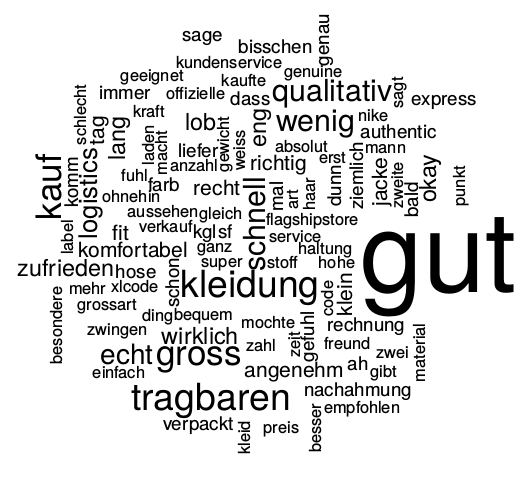
\includegraphics[width=\linewidth]{empirische_ergebnisse/wortwolke_cn}
    \endminipage\hfill
    \minipage{0.5\textwidth}
    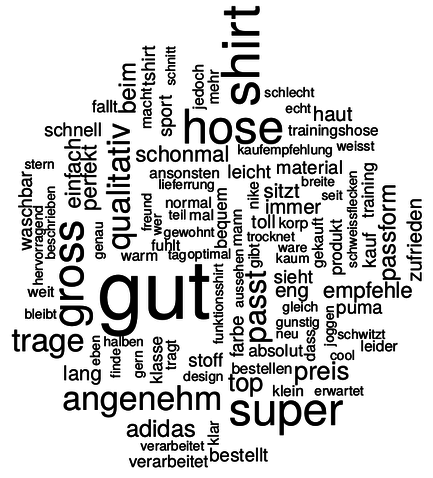
\includegraphics[width=\linewidth]{empirische_ergebnisse/wortwolke_de}
    \endminipage        
    %%\fbox{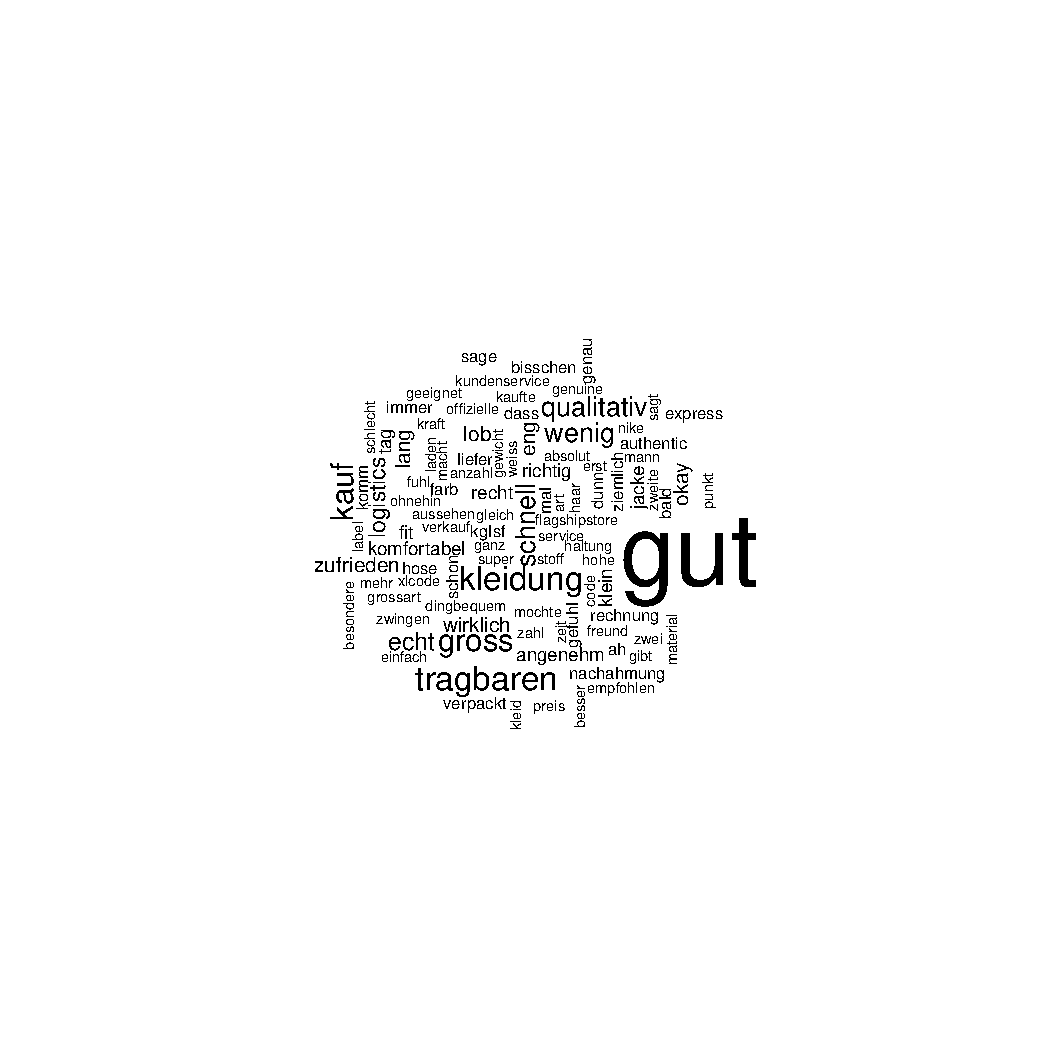
\includegraphics[page=1, scale=0.5]{empirische_ergebnisse/gesammt_cn.pdf}}   
    %%\hspace{30px}
    %%\fbox{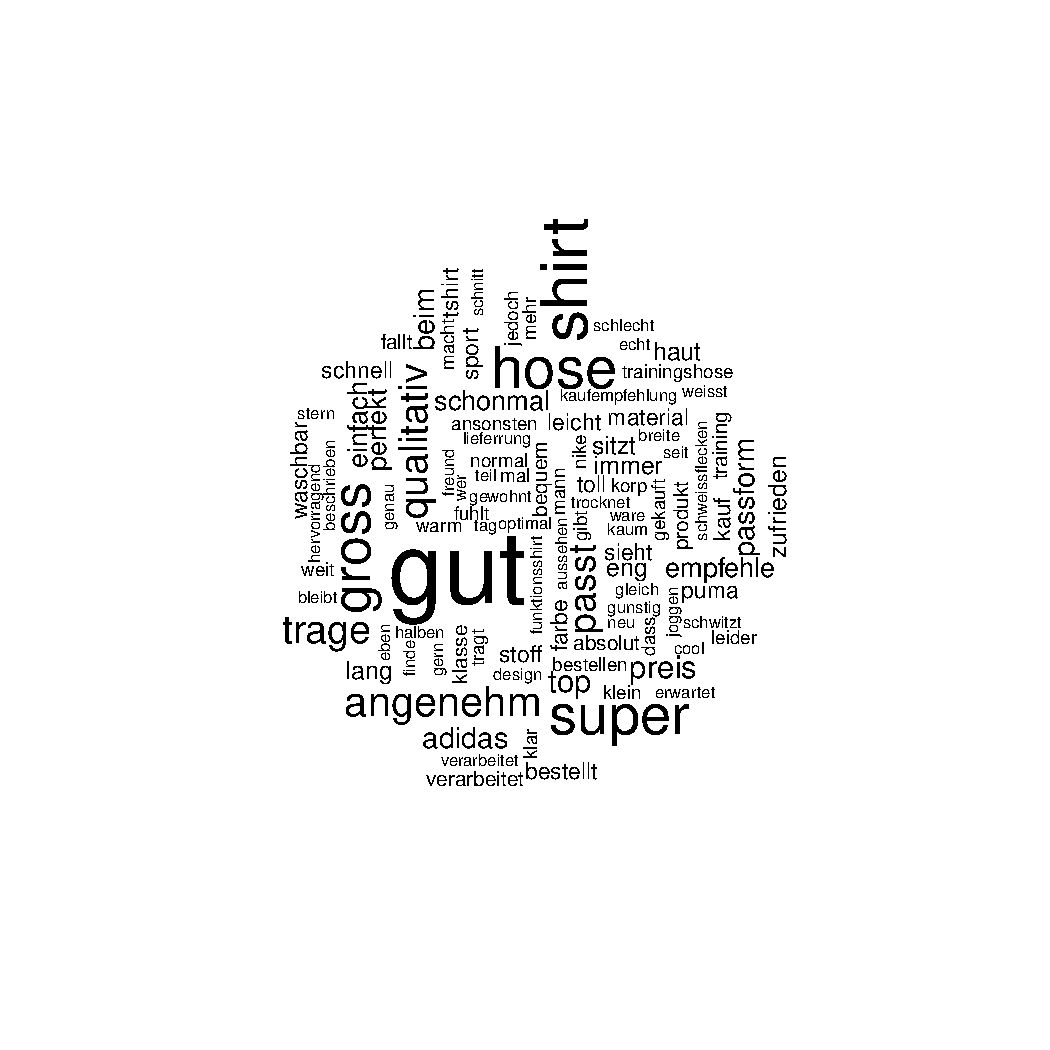
\includegraphics[page=1, scale=0.5]{empirische_ergebnisse/gesammt_de.pdf}}   
    \caption[die Wortwolken von chinesischen (Links) sowie deutschen (Rechts) OCRs]{die Wortwolken von chinesischen (Links) sowie deutschen (Rechts) \ac{OCRs} (Quelle: Eigene Darstellung)}
    \label{fig:wortwolke}
\end{figure}

Die beiden Wortwolken sind die Wörtern aufzubauen, von denen die Menge des Auftretens größer als ein Promille der Menge von chinesischen oder deutschen \ac{OCRs} ist. Von Abbildung \ref{fig:wortwolke} kann man wissen, dass die Kleidungen von allen Marken in beiden Ländern als ``gut'' bewertet wurden. Worum die Kunden sich zuerst kümmern sind die Größe, Tragbarkeit, und Qualität. Die chinesischen Kunden ziehen die Logistik Dienstleistung in Erwägung aber die Deutschen berücksichtigen den Preis mehr. Diese Gemeinsamkeiten und Unterschiede kann man auch durch die Top 10 Wörter in Abbildung \ref{fig:top10} zusammenfassen.

\begin{figure}[htb]
    \fbox{\includegraphics[page=2, scale=0.45]{empirische_ergebnisse/gesammt_cn.pdf}}    
    \fbox{\includegraphics[page=2, scale=0.45]{empirische_ergebnisse/gesammt_de.pdf}}   
    \caption[die Top 10 Wörter von chinesischen (Links) sowie deutschen (Rechts) OCRs]{die Top 10 Wörter von chinesischen (Links) sowie deutschen (Rechts) \ac{OCRs} (Quelle: Eigene Darstellung)}
    \label{fig:top10}
\end{figure}

Von diesen chinesischen Top 10 Wörtern, sieht man auch, dass die chinesischen Kunden viel mehr das Wort ``gut'' verwenden wollen als die Deutschen. Das kann auch das Problem von maschineller Übersetzung sein. Außerdem beachten die Chinesen die Logistik (``logistics'', ``schnell'') und ob die Waren zertifiziert sind (``echt''), während die Deutschen das Gefühl der Aussicht oder den Preis mehr berücksichtigen (``angenehm'', ``passt'', ``preis'').

Die deutschen Reviews werden in dem Zeitraum von 7. Januar 2012 bis 9. Mai 2015 geschrieben, und die Chinesen haben die Kommentaren zwischen 10. Februar 2014 und 2. Juni 2015 geschrieben. Dieser Datensammlungsprozess ist genau am 2. Juni 2015 durchgeführt worden. Das heißt: die Chinesen wollen gern \ac{OCRs} schreiben aber die deutschen Kunden wollen vielleicht nicht so.

In den Abschnitten \ref{sec:h0} bis \ref{sec:h4} wird jede Hypothese in unterschiedlichen Kategorien und Marken getestet. Danach wird sie in allgemeiner Hinsicht zusammengefasst. Eine geschlechtsspezifische Analyse wird nicht in dieser Arbeit auf folgenden Gründen erstellt:
\begin{enumerate}
	\item  Wie es in Abschnitt \ref{sec:OCRsinTextil} geschrieben steht, waren die demographischen Variablen wie Alter und Geschlecht in keinem Zusammenhang mit Online-Bekleidungseinkauf \citep{Goldsmith2002}.
	\item Die Kunden sind anonym im Internet. Durch die \ac{OCRs} ist es unsichtbar über das Geschlecht. Es ist nicht so gewissenschaft zu sagen, dass die Frauen nur die weiblichen Produkten kaufen wollen.
	\item Die Abbildung \ref{fig:sechsdimensionen} zeigt, dass die Dimension: ``Maskulinität gegenüber Femininität'' von Deutschland und China gleiche Punkte hat. Das heißt: Die geschlechtspezifische Auswirkung zwischen Deutschland und China in kulturellem Bereich ist gleich, deshalb braucht man diese nicht zu unterscheiden.
\end{enumerate}
Die folgende Tabelle \ref{tab:jeweil_preis} zeigt den Preis des jeweiligen Produkts in beiden Ländern. Daran sieht man, dass der Preis des Produkts in China und Deutschland keinen großen Unterschied hat. Und laut \citet{lu2015understanding} sind die Forschungsergebnisse für die Wichtigkeit des Preis inkonsistent. Deshalb wird der Faktor von dem Preis in dieser Arbeit nicht berücksichtigen.
\begin{table}[htb]
\centering
\begin{tabular}{|c|c|c|}
\hline
Produkt                                                   & Deutschland & China \\ \hline
\begin{tabular}[c]{@{}c@{}}Adidas\\ männlich\end{tabular} & \EUR{29,99}            & CNY 199 ($\approx$ \EUR{29,70})      \\ \hline
\begin{tabular}[c]{@{}c@{}}Adidas\\ weiblich\end{tabular} & \EUR{34,99}            & CNY 250 ($\approx$ \EUR{37,31})       \\ \hline
Nike                                                      & \EUR{56}            & CNY 359 ($\approx$ \EUR{53,58})       \\ \hline
Puma                                                      & \EUR{16,98}            & CNY 119 ($\approx$ \EUR{17,76})       \\ \hline
\end{tabular}
\caption[Der jeweilige Preis von jeder Kleidung in Deutschland und China]{Der jeweilige Preis von jeder Kleidung in Deutschland und China (Datenquelle von \href{http://www.amazon.de/}{Amazon} und \href{https://www.tmall.com/}{Tmall}, Euro gegenüber dem CNY-Wechselkurs von \href{http://www.boc.cn/sourcedb/whpj/}{Bank of China}: 6,70, am 2. Juni 2015)}
\label{tab:jeweil_preis}
\end{table}
%%=======================================
\section{Hypothesenüberprüfung} \label{sec:h0}
%%=======================================
Die Nullhypothese handelt sich um die wesentliche Frage, ob es kulturelle Einflüsse auf den quantitativen und qualitativen \ac{OCRs} gibt. Wenn es keine Einflüsse darauf gibt, sollte die quantitativen und qualitativen Valenzen beiden normalverteilt sind. 

In dieser Arbeit wird der Shapiro-Wilk-Test durchgeführt. Der Shapiro-Wilk-Test ist ein statistischer Signifikanztest, der die Hypothese überprüft, dass die zugrunde liegende Grundgesamtheit einer Stichprobe normalverteilt ist. Die Nullhypothese $H_0$ nimmt an, dass eine Normalverteilung der Grundgesamtheit vorliegt. Wird alternativ der p-Wert des Tests ermittelt, so wird die Nullhypothese in der Regel nicht abgelehnt, wenn der p-Wert größer ist als das festgelegte Signifikanzniveau $\alpha$. Der Test kann zum Überprüfen von univariaten Stichproben mit 3 bis 5000 Beobachtungen eingesetzt werden. \citep{SHAPIRO01121965}

Nach \citet[p.~547]{patrick1995remark} ist die Hypothese $H_0$ abgelehnt wenn der p-Wert kleiner als 0,1 ist. Tabelle \ref{tab:h0_pwert} zeigt die Ergebnisse für die beiden Ländern. 
\begin{table}[htb]
\centering
\begin{tabular}{|l|l|l|}
\hline
p-Wert      & quantitative \ac{OCRs} & qualitative \ac{OCRs}  \\\hline
China       & $<2.2 \times 10^{-16}$ &  $<2.2 \times 10^{-16}$  \\\hline
Deutschland &  $<2.2 \times 10^{-16}$  & 0.003672        \\ \hline
\end{tabular}
\caption[Die Ergebnisse durch Shapiro-Wilk-Test für China und Deutschland]{Die Ergebnisse durch Shapiro-Wilk-Test für China und Deutschland (Quelle: Eigene Darstellung)}
\label{tab:h0_pwert}
\end{table}
\begin{figure}[htb]
    \minipage{0.5\textwidth}
    \includegraphics[page=2,width=\linewidth]{empirische_ergebnisse/gesammt_cn_sentiment.pdf}
    \endminipage\hfill
    \minipage{0.5\textwidth}
    \includegraphics[page=2,width=\linewidth]{empirische_ergebnisse/gesammt_de_sentiment.pdf}
    \endminipage        
\caption[Das Q-Q-Plot der quantitativen Valenzen für China und Deutschland]{Das Q-Q-Plot der quantitativen Valenzen für China (Links) und Deutschland (Rechts) Quelle: Eigene Darstellung}
\label{fig:qqplot_quantitativ}
\end{figure}
\begin{figure}[htb]
    \minipage{0.5\textwidth}
    \includegraphics[page=3,width=\linewidth]{empirische_ergebnisse/gesammt_cn_sentiment.pdf}
    \endminipage\hfill
    \minipage{0.5\textwidth}
    \includegraphics[page=3,width=\linewidth]{empirische_ergebnisse/gesammt_de_sentiment.pdf}
    \endminipage        
\caption[Das Q-Q-Plot der qualitativen Valenzen für China und Deutschland]{Das Q-Q-Plot der qualitativen Valenzen für China (Links) und Deutschland (Rechts) Quelle: Eigene Darstellung}
\label{fig:qqplot_qualitativ}
\end{figure}

Aus dieser Tabelle kann man sehen, dass die alle vier p-Werte kleiner als 0,1 sind. Mit dem Quantile-Quantile-Plot (Q-Q-Plot) kann man die empirischen Häufigkeitsverteilung mit der hypothetischen Verteilung \ac{bzw.} Normalverteilung vergleichen. Die Abbildungen \ref{fig:qqplot_quantitativ} und \ref{fig:qqplot_qualitativ} zeigen die Q-Q-Plot der quantitativen und qualitativen Valenzen graphisch aus. Besonders in dem Q-Q-Plot der deutschen qualitativen Valenz sind die Verteilung sehr ähnlich wie die Normalverteilung, aber der p-Wert davon zeigt anders aus. Durch diesen Abbildungen und Tabelle \ref{tab:h0_pwert} wird die Hypothese $H_0$ abgelehnt. Anders gesagt, es gibt tätsachlich kulturellen Einflüsse auf quantitativen und qualitativen \acl{OCRs}. 

Nur mit diesem Ergebnis kann man die weiteren Hypothesen testen. In Abschnitt \ref{sec:hypothese} werden vier Attribute der \ac{OCRs} an der quantitativen und qualitativen Seite erstellt. Die Hypothesen \ref{hyp:1} bis \ref{hyp:4} testen, ob es kulturelle Einflüsse auf die vier Attribute gibt. In den Abschnitten \ref{sec:h1} bis \ref{sec:h4} sind die empirischen Ergebnisse.
%%=======================================
\section{Hypothese 1} \label{sec:h1}
%%=======================================
Hypothese \ref{hyp:1} handelt sich um die Frage, ob es kulturellen Einflüsse auf die Menge und Länge der \ac{OCRs} gibt. In diesem Abschnitt wird Hypothese \ref{hyp:1} in Allgemeinen \ac{bzw.} auch in verschiedenen Kategorien (T-Shirt und Hose) und Marken (Adidas, Nike, Puma) getestet. Damit kann man nicht nur kennen, ob Hypothese \ref{hyp:1} in allgemeiner Hinsicht unterstützt wird, sondern auch in verschiedenen Situationen.
%%=======================================
\subsection{Hypothese 1 in unterschiedlichen Kategorien}
%%=======================================
Insgesamt wurden 2402 chinesischen \ac{OCRs} über T-Shirt gesammelt, während es bei den deutschen nur 98 sind. Über Hose, wurden 266 mal chinesischen \ac{OCRs} gesammelt und 70 mal deutsche. Tabelle \ref{tab:volumenTshirtHose} zeigt die Ergebnisse.
\begin{table}[htb]
\centering
\begin{tabular}{|llll|}
\hline
\multicolumn{1}{|l|}{T-Shirt}     & \multicolumn{1}{l|}{Wörter} & \multicolumn{1}{l|}{Zeichen} & Menge \\ \hline
\multicolumn{1}{|l|}{China}       & \multicolumn{1}{l|}{22255}  & \multicolumn{1}{l|}{139258}  & 2402   \\ \hline
\multicolumn{1}{|l|}{Deutschland} & \multicolumn{1}{l|}{3821}   & \multicolumn{1}{l|}{24039}   & 98     \\ \hline
                                  &                             &                              &        \\ \hline
\multicolumn{1}{|l|}{Hose}        & \multicolumn{1}{l|}{Wörter} & \multicolumn{1}{l|}{Zeichen} & Menge \\ \hline
\multicolumn{1}{|l|}{China}       & \multicolumn{1}{l|}{2744}   & \multicolumn{1}{l|}{17021}   & 266   \\ \hline
\multicolumn{1}{|l|}{Deutschland} & \multicolumn{1}{l|}{2411}   & \multicolumn{1}{l|}{14658}   & 70     \\ \hline
\end{tabular}
\caption[Das Volumen der OCRs über T-Shirt und Hose von qualitativen und quantitativen Seiten]{Das Volumen der \ac{OCRs} über T-Shirt und Hose von qualitativen und quantitativen Seiten (Quelle: Eigene Darstellung)}
\label{tab:volumenTshirtHose}
\end{table}


Man kann einfach rausrechnen, dass die chinesischen Kunden durchschnittlich weniger Wörter benutzt haben als die deutschen. Im Durchschnitt benutzt ein chinesischer Kunde nur 9 bis 10 Wörtern während der deutsche Kunden 34 bis 39 benutzt hat. Das heißt: die chinesischen \ac{OCRs} haben meistens nur einen Satz und die Deutschen schreiben mehreren Sätzen. Durch diese Daten kann man auch einfach das durchschnittliches Volumen rausrechnen. Dieses Volumen wird in Abbildung \ref{fig:durchschnittlichesVolumen} vergliechen.
\begin{figure}[htb]
\centering
    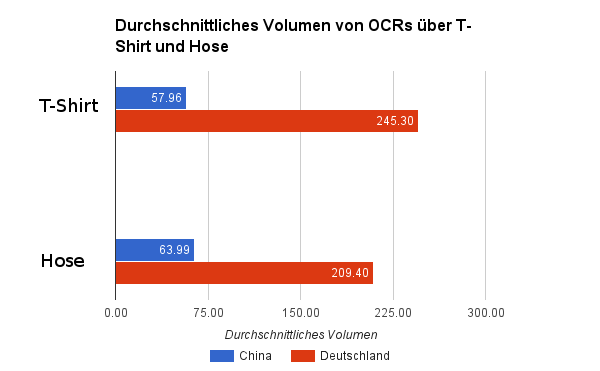
\includegraphics[width=\textwidth]{empirische_ergebnisse/hypothese1volumen} 
    \caption[Durchschnittliches Volumen von qualitativen OCRs über T-Shirt und Hose]{Durchschnittliches Volumen von qualitativen \ac{OCRs} über T-Shirt und Hose (Quelle: Eigene Darstellung)}
    \label{fig:durchschnittlichesVolumen}
\end{figure}

Aus dieser Abbildung kann man schon erfassen, dass das deutsche durchschnittliche Volumen drei bis vier mal so groß wie das Chinesische ist. Das entspricht auch die Anzahl von Wörtern. Das heißt: Im Durchschnitt schreiben die deutschen Kunden drei bis vier Sätzen, während die Chinesen nur einen Satz schreiben, aber sie schreiben \ac{OCRs} gerne nach dem Kauf. Deshalb wird Hypothese \ref{hyp:1} im Bereich \ac{OCRs} von T-Shirt und Hose nur in dem qualitativen Aspekt gestützt.
%%=======================================
\subsection{Hypothese 1 bei unterschiedlichen Marken}
%%=======================================
Wie es vorher geschrieben wurde, wurden die Daten aus insgesamt drei unterschiedlichen Marken gesammelt, die ``Adidas'', ``Nike'' und ``Puma'' sind. Tabelle \ref{tab:volumenMarken} zeigt das Volumen der qualitativen \ac{OCRs} von den drei Marken.
\begin{table}[htb]
\centering
\begin{tabular}{|llll|}
\hline
\multicolumn{1}{|l|}{Adidas}      & \multicolumn{1}{l|}{Wörter} & \multicolumn{1}{l|}{Zeichen} & Menge \\ \hline
\multicolumn{1}{|l|}{China}       & \multicolumn{1}{l|}{2744}   & \multicolumn{1}{l|}{17021}   & 266    \\ \hline
\multicolumn{1}{|l|}{Deutschland} & \multicolumn{1}{l|}{2411}   & \multicolumn{1}{l|}{14658}   & 70     \\ \hline
                                  &                             &                              &        \\ \hline
\multicolumn{1}{|l|}{Nike}        & \multicolumn{1}{l|}{Wörter} & \multicolumn{1}{l|}{Zeichen} & Menge \\ \hline
\multicolumn{1}{|l|}{China}       & \multicolumn{1}{l|}{17541}  & \multicolumn{1}{l|}{109589}  & 1923   \\ \hline
\multicolumn{1}{|l|}{Deutschland} & \multicolumn{1}{l|}{1909}   & \multicolumn{1}{l|}{12023}   & 40     \\ \hline
                                  &                             &                              &        \\ \hline
\multicolumn{1}{|l|}{Puma}        & \multicolumn{1}{l|}{Wörter} & \multicolumn{1}{l|}{Zeichen} & Menge \\ \hline
\multicolumn{1}{|l|}{China}       & \multicolumn{1}{l|}{4714}   & \multicolumn{1}{l|}{29669}   & 479    \\ \hline
\multicolumn{1}{|l|}{Deutschland} & \multicolumn{1}{l|}{1912}   & \multicolumn{1}{l|}{12016}   & 58     \\ \hline
\end{tabular}
\caption[Das Volumen der OCRs bei verschiedenen Marken]{Das Volumen der \ac{OCRs} bei verschiedenen Marken (Quelle: Eigene Darstellung)}
\label{tab:volumenMarken}
\end{table}

Durch Tabelle \ref{tab:volumenMarken} steht es fest, dass die Menge der chinesischen \ac{OCRs} bei jeder Marke größer als die von den Deutschen ist. Bei der Marke ``Nike'' ist die Menge von den chinesischen \ac{OCRs} sogar fast das 50fache wie die der Deutschen. Bei der Marke ``Adidas'' ist die Menge der Wörtern von chinesischen und deutschen fast gleich, trotz der Tatsache dass die chinesischen \ac{OCRs} drei mal mehr als die deutschen \ac{OCRs} sind. Folgende Abbildung \ref{fig:volumenMarken} zeigt den großen Unterschied.
\begin{figure}[htb]
\centering
    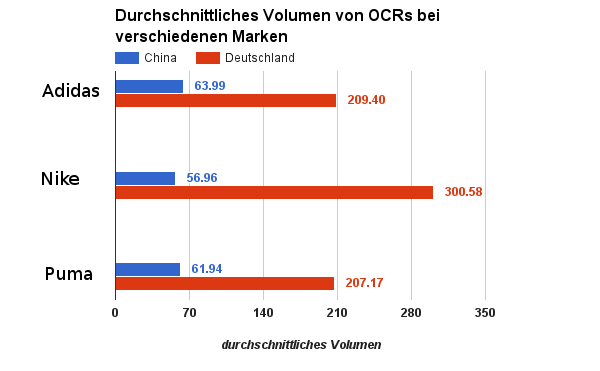
\includegraphics[width=\textwidth]{empirische_ergebnisse/volumenMarken} 
    \caption[Durchschnittliches Volumen von qualitativen OCRs bei verschiedenen Marken]{Durchschnittliches Volumen von qualitativen \ac{OCRs} bei verschiedenen Marken (Quelle: Eigene Darstellung)}
    \label{fig:volumenMarken}
\end{figure}

Daran sieht man dass die chinesischen Kunden beim Online-Einkauf bei diesen drei Marken nur ungefähr 60 Charaktere in den \ac{OCRs} schreiben, aber die Deutschen schreiben mehr, von 200 bis 300 Charaktere. Besonders schreiben die deutschen Kunden von Nike mehr als die von den anderen zwei Marken. Dieses Ergebnis ist ähnlich wie das Ergebnis in Abbildung \ref{fig:durchschnittlichesVolumen}. Die deutschen Kunden schreiben längere aber wenigere \ac{OCRs} als die chinesischen Kunden. Das heißt, dass Hypothese \ref{hyp:1} bei unterschiedlichen Marken auch nur in dem qualitativen Aspekt gestützt wird. 
%%=======================================
\subsection{Hypothese 1 im Allgemeinen}
%%=======================================
Weil die Hypothese \ref{hyp:1} in den beiden Kategorien und allen drei verschiedenen Marken im quantitativen Aspekt abgelehnt aber im qualitativen Aspekt gestützt wird, wird es vorgeschlagen, dass die Hypothese \ref{hyp:1} in der gleichen Situation in allgemeiner Weise ist. Tabelle \ref{tab:volumenAllgemeinen} zeigt das allgemeine Ergebnis aus.
\begin{table}[htb]
\centering
\begin{tabular}{|l|l|l|l|}
\hline
            & Wörter & Zeichen & Menge \\ \hline
China       & 24999 & 156279  & 2668   \\ \hline
Deutschland & 6232   & 38697   & 168    \\ \hline
\end{tabular}
\caption[Das Volumen der OCRs im Allgemeinen von qualitativen und quantitativen Seiten]{Das Volumen der \ac{OCRs} im Allgemeinen von qualitativen und quantitativen Seiten (Quelle: Eigene Darstellung)}
\label{tab:volumenAllgemeinen}
\end{table}

Aus dieser Tabelle kann man erfassen, dass bei den chinesischen \ac{OCRs} nur 9,37 Wörtern (58,58 Zeichen) durchschnittlich benutzt werden, aber die deutschen Kunden schreiben 37,10 Wörtern (230,34 Zeichen) im Durchschnitt. Abbildung \ref{fig:volumenAllgemeinen} zeigt das Ergebnis graphisch.
\begin{figure}[htb]
\centering
    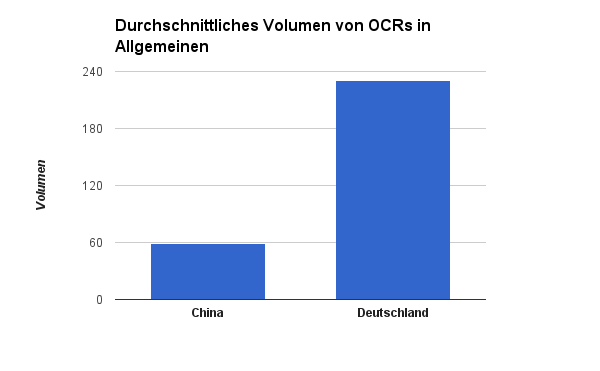
\includegraphics[width=\textwidth]{empirische_ergebnisse/volumenAllgemeinen} 
    \caption[Durchschnittliches Volumen von qualitativen OCRs]{Durchschnittliches Volumen von qualitativen \ac{OCRs} (Quelle: Eigene Darstellung)}
    \label{fig:volumenAllgemeinen}
\end{figure}

Die meinsten chinesischen \ac{OCRs} haben nur einen oder zwei Wörtern, sowie: ``gut'', ``zufrieden'', ``Lob'', ``Okay'', \ac{usw}. Aber die Deutschen schreiben mehr. %%Wer mehr schreibt, teilt mehr und gerne die Information. Deshalb sind die chinesischen Kunden zurückhaltender beim Informationsaustausch als die Deutschen. Nach \citet{Lam2009} liegt dies daran, weil die Chinesen in einer Kultur mit großer Machtdistanz leben. 

Wegen der kollektivistischen Kultur bevorzugen die chinesischen Kunden, nacheinander die \ac{OCRs} zu schreiben, wenn es schon große Menge von \ac{OCRs} gibt. Deshalb sieht man in Tabelle \ref{tab:volumenMarken}, dass es fast 2000 \ac{OCRs} für die Marke ``Nike'' gibt während es nur 266 Reviews für ``Adidas'' sind. 

Zusammengefasst sind die chinesischen Reviews deutlich kürzer, aber mehr als die deutschen Reviews. Das heißt: In Quantität sind die chinesischen \ac{OCRs} viel mehr als die deutschen, aber in Qualität sind die deutschen \ac{OCRs} viel besser. Die Hypothese \ref{hyp:1} wird in dem quantitativen Aspekt abgelehnt aber in dem qualitativen Aspekt gestützt.
%%=======================================
\section{Hypothese 2}
%%=======================================
Hypothese \ref{hyp:2} wird in dieser Arbeit vorgeschalgen, um die Valenz der quantitativen und qualitativen \ac{OCRs} zu unterscheiden und zwischen den beiden Ländern zu vergleichen. Damit wird sie, ähnlich wie Hypothese \ref{hyp:1}, in unterschiedlichen Kategorien und Marken diskutiert.
%%=======================================
\subsection{Hypothese 2 in unterschiedlichen Kategorien}
%%=======================================
Wie es in Abschnitt \ref{sec:h1} geschrieben wird, haben die Daten in zwei Kategorien unterschiedlichen Mengen. Deshalb ist es besser,  die Analyse getrennt für T-Shirt und Hose durchzuführen.

\begin{figure}[htb]
%\centering
    {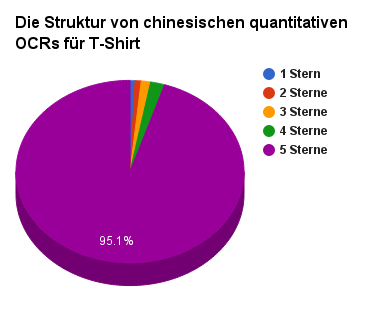
\includegraphics[width=0.5\textwidth]{empirische_ergebnisse/struktur_cn_quantitativ_Tshirt}}    
    {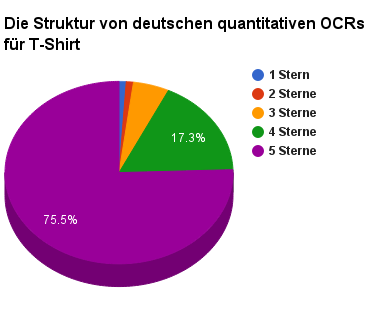
\includegraphics[width=0.5\textwidth]{empirische_ergebnisse/struktur_de_quantitativ_Tshirt}}   
    \caption[Die Struktur von chinesischen und deutschen quantitativen OCRs über T-Shirt]{Die Struktur von chinesischen (Links) und deutschen (Rechts) quantitativen \ac{OCRs} über T-Shirt (Quelle: Eigene Darstellung)}
    \label{fig:struktur_quantitativ_Tshirt}
\end{figure}

Abbildung \ref{fig:struktur_quantitativ_Tshirt} zeigt die Struktur der \ac{OCRs} über T-Shirt von quantitativer Sicht in den beiden Ländern. Dort kann man erkennen, dass die Mehrheit der \ac{OCRs} von den beiden Ländern fünf Sterne für das T-Shirt ist. Aber der Unterschied ist auch sichtbar. Die chinesischen Kunden geben viel lieber fünf Sterne als die Deutschen. 95\% von den chinesischen \ac{OCRs} sind fünf Sterne, aber bei der Deutschen ist die Zahl nur 75\%. Das heißt auch, dass die chinesischen quantitativen \ac{OCRs} viel dichter als die deutschen sind.

\begin{figure}[htb]
    \minipage{0.5\textwidth}
    \includegraphics[page=4,width=\linewidth]{empirische_ergebnisse/Tshirt_cn_sentiment.pdf}
    \endminipage\hfill
    \minipage{0.5\textwidth}
    \includegraphics[page=4,width=\linewidth]{empirische_ergebnisse/Tshirt_de_sentiment.pdf}
    \endminipage 
%\centering
    \caption[Die Verteilung der Valenzen von chinesischen und deutschen qualitativen OCRs für T-Shirt]{Die Verteilung der Valenzen von chinesischen und deutschen qualitativen \ac{OCRs} für T-Shirt (Quelle: Eigene Darstellung)}
    \label{fig:valenz_Tshirt}
\end{figure}

Lässt sich der Abbildung \ref{fig:valenz_Tshirt} entnehmen, dass die Valenzen von chinesischen qualitativen \ac{OCRs} viel dichter und zentralisierter als die von Deutschen sind. Die chinesischen qualitativen OCRs haben zwei großen Gruppen aber die deutschen Polaritäten sind vielfähig und dezentralisiert. Nach der Hinsicht in den Rohdaten ist es klar, dass die beiden Valenzen von den zwei großen Gruppen die Werte 0 und 0,3716 festsetzen. Durch das Lexikon weiß man, dass die Polarität des Wortes “gut” 0,3716 ist. Polarität 0 bei chinesischen OCRs tritt 589 mal auf, und 0,3716 tritt 502 mal auf. Das heißt auch, dass die chinesischen Kunden meistens kein Gefühl ausgedrückt oder nur “gut” geschrieben haben, aber die deutschen Kunden schreiben mehr über das eigene Gefühl über das T-Shirt. Die blauen Linien sind die entsprechende Normalverteilung. Aus der Abbildung geht hervor, dass die Valenzen nicht normal verteilt werden.

\begin{figure}[htb]
%\centering
    {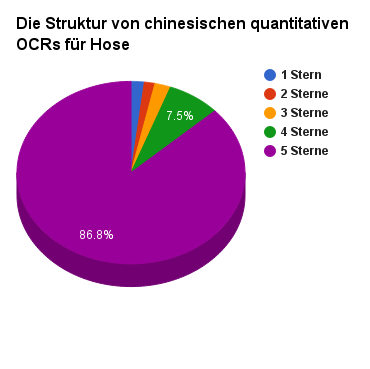
\includegraphics[width=0.5\textwidth]{empirische_ergebnisse/struktur_cn_quantitativ_Hose}}    
    {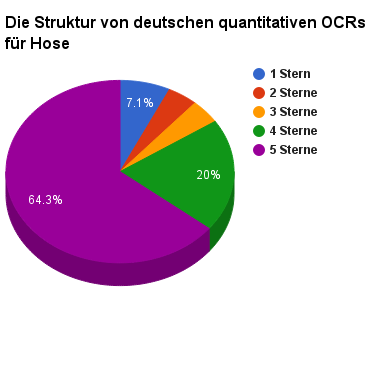
\includegraphics[width=0.5\textwidth]{empirische_ergebnisse/struktur_de_quantitativ_Hose}}   
    \caption[Die Struktur von chinesischen und deutschen quantitativen OCRs über Hose]{Die Struktur von chinesischen (Links) und deutschen (Rechts) quantitativen \ac{OCRs} über Hose (Quelle: Eigene Darstellung)}
    \label{fig:struktur_quantitativ_Hose}
\end{figure}

Für die Hosen ist das Ergebnis graphisch fast gleich. Abbildung \ref{fig:struktur_quantitativ_Hose} zeigt dass über 86\% der chinesischen Kunden fünf Sterne für die Hosen geben aber die Zahl von den Deutschen ist nur 64,3\%. Aus der Abbildung \ref{fig:valenz_Hose} geht hervor, dass 24,81\% der chinesischen Kunden kein Wort über das Gefühl gegeben haben und 14,29\% der Chinesen nur ``gut'' geschrieben haben.Aber wie die deutschen Kunden in Abbildung \ref{fig:valenz_Tshirt} sind, bleiben hier die Deutschen in der Abbildung \ref{fig:valenz_Hose} dezentralisiert.
\begin{figure}[htb]
%\centering
    \minipage{0.5\textwidth}
    \includegraphics[page=4,width=\linewidth]{empirische_ergebnisse/hose_cn_sentiment.pdf}
    \endminipage\hfill
    \minipage{0.5\textwidth}
    \includegraphics[page=4,width=\linewidth]{empirische_ergebnisse/hose_de_sentiment.pdf}
    \endminipage 
    \caption[Die Verteilung der Valenzen von chinesischen und deutschen qualitativen OCRs für Hose]{Die Verteilung der Valenzen von chinesischen und deutschen qualitativen \ac{OCRs} für Hose (Die blauen Linien sind die entsprechende Normalverteilung.) (Quelle: Eigene Darstellung)}
    \label{fig:valenz_Hose}
\end{figure}

Weil die chinesischen Kunden wesentlich mehr ``fünf Sterne'' ausgegeben haben als die Deutschen (durch Abbildung \ref{fig:struktur_quantitativ_Tshirt} und \ref{fig:struktur_quantitativ_Hose}), ist es natürlich, dass die durchschnittliche Valenz der deutschen quantitativen \ac{OCRs} kleiner als die von den chinesischen ist. Das heißt: An der Seite der quantitativen \ac{OCRs}, ist die Valenz von den Chinesischen besser als die von Deutschen.

Aber die Tabelle \ref{tab:valenzKategorien} zeigt Etwas anderes an der Seite der qualitativen \ac{OCRs}. Die chinesischen qualitativen Valenzen sind in beiden Kategorien kleiner als die von den Deutschen. Das heißt: Basierend auf dem gleichen Produkt drücken die deutschen Kunden sich selbst mehr positiv aus, als die Chinesen, obwohl sie schlechte Sterne ausgegeben haben. Die Tabelle bestätigt die Begründung 3 am Ende des Abschnitts \ref{sec:auswirkung}. Zusammenfassend wird die Hypothese \ref{hyp:2} in unterschiedlichen Kategorien \ac{bzw.} T-Shirt und Hose in dieser Arbeit nur an der qualitativen Seite gestützt.

\begin{table}[htb]
\centering
\begin{tabular}{|c|c|c|c|c|}
\hline
\multirow{2}{*}{} & \multicolumn{2}{c|}{quantitative Valenz} & \multicolumn{2}{c|}{qualitative Valenz} \\ \cline{2-5} 
                  & China             & Deutschland          & China             & Deutschland         \\ \hline
T-Shirt           & 4,898876          & 4,653061             & 0,2579923         & 0,7124276           \\ \hline
Hose              & 4,759398          & 4,3                  & 0,2023165         & 0,6110686           \\ \hline
\end{tabular}
\caption[Die Valenz von quantitativen und qualitativen OCRs über unterschiedlichen Kategorien in beiden Ländern]{Die Valenz von quantitativen und qualitativen \ac{OCRs} über unterschiedlichen Kategorien in beiden Ländern (Quelle: Eigene Darstellung)}
\label{tab:valenzKategorien}
\end{table}


%%=======================================
\subsection{Hypothese 2 bei unterschiedlichen Marken}
%%=======================================
In diesem Abschnitt wird die Hypothese \ref{hyp:2} bei den drei ausgewählten Marken getestet. Weil die beiden Hosen von Adidas produziert werden, sind die Ergebnisse von Adidas gleich wie die Ergebnisse von den Hosen. Deshalb repräsentieren die Abbildungen \ref{fig:struktur_quantitativ_Hose} und \ref{fig:valenz_Hose} auch die Ergebnisse von der Marke ``Adidas''. Die Ergebnisse von den anderen zwei Marken werden nicht wie Abbildungen \ref{fig:struktur_quantitativ_Tshirt} oder \ref{fig:valenz_Tshirt} national verglichen, sondern bei unterschiedlichen Marken im einzelnen Land verglichen. Damit wird getestet, ob die Ergebnisse wirklich stabil oder nur im Durchschnitt stabil sind.

\begin{figure}[htb]
%\centering
    {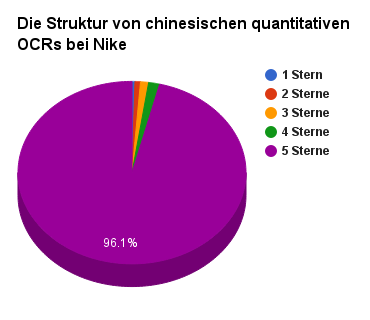
\includegraphics[width=0.5\textwidth]{empirische_ergebnisse/struktur_cn_quantitativ_nike}}    
    {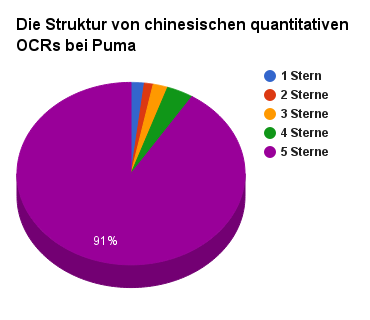
\includegraphics[width=0.5\textwidth]{empirische_ergebnisse/struktur_cn_quantitativ_puma}}   
    \caption[Die Struktur von chinesischen quantitativen OCRs bei Nike und Puma]{Die Struktur von chinesischen quantitativen \ac{OCRs} bei Nike und Puma (Quelle: Eigene Darstellung)}
    \label{fig:struktur_cn_nike_puma}
\end{figure}

\begin{figure}[h]
    \minipage{0.5\textwidth}
    \includegraphics[page=4,width=\linewidth]{empirische_ergebnisse/nike_cn_sentiment.pdf}
    \endminipage\hfill
    \minipage{0.5\textwidth}
    \includegraphics[page=4,width=\linewidth]{empirische_ergebnisse/puma_cn_sentiment.pdf}
    \endminipage 
    \caption[Die Verteilung der chinesischen Valenzen von qualitativen OCRs bei zwei unterschiedlichen Marken]{Die Verteilung der chinesischen Valenzen von qualitativen \ac{OCRs} bei zwei unterschiedlichen Marken (Die blauen Linien sind die entsprechende Normalverteilung.) (Quelle: Eigene Darstellung)}
    \label{fig:valenz_cn_marken}
\end{figure}

Durch die Abbildungen \ref{fig:struktur_cn_nike_puma} und \ref{fig:valenz_cn_marken} kann man erfassen, dass über 90\% der chinesischen quantitativen \ac{OCRs} 5 Sterne sind, und viele chinesischen Kunden sagen nichts ihr Gefühl aus oder schreiben einfach nur ein ``Gut''. Diese Ergebnisse sind gleich wie die Ergebnisse von den chinesischen \ac{OCRs} über T-Shirt und Hose. Damit meint man: Die Ergebnisse für unterschiedlichen Kategorien sind stabil für die Chinesen auch bei unterschiedlichen Marken.

Die deutschen Ergebnisse von den zwei Marken werden durch Abbildungen \ref{fig:struktur_de_nike_puma} und \ref{fig:valenz_de_marken} gezeigt. Von den Abbildungen sieht man dass die deutschen Ergebnisse sich nicht ändern. Ungefähr 75\% von den deutschen Kunden geben ``fünf Sterne'' aus, und die Valenzen von deutschen qualitativen \ac{OCRs} sind voneinander getrennt. Besonders bei Puma gibt es noch keine quantitative Bewertung, die einen Stern oder zwei Sterne hat.

\begin{figure}[htb]
%\centering
    {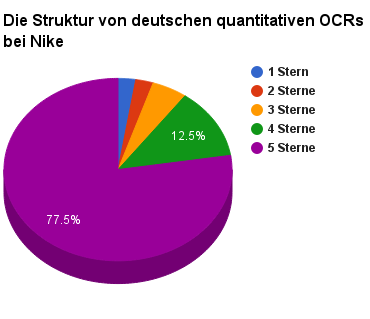
\includegraphics[width=0.5\textwidth]{empirische_ergebnisse/struktur_de_quantitativ_nike}}    
    {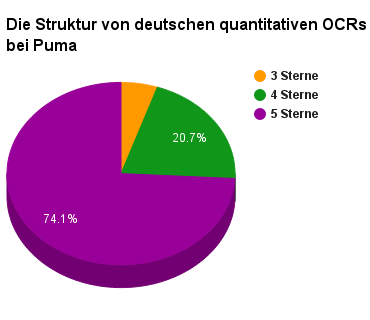
\includegraphics[width=0.5\textwidth]{empirische_ergebnisse/struktur_de_quantitativ_puma}}   
    \caption[Die Struktur von deutschen quantitativen OCRs bei Nike und Puma]{Die Struktur von deutschen quantitativen \ac{OCRs} bei Nike und Puma (Quelle: Eigene Darstellung)}
    \label{fig:struktur_de_nike_puma}
\end{figure}

\begin{figure}[h]
    \minipage{0.5\textwidth}
    \includegraphics[page=4,width=\linewidth]{empirische_ergebnisse/nike_de_sentiment.pdf}
    \endminipage\hfill
    \minipage{0.5\textwidth}
    \includegraphics[page=4,width=\linewidth]{empirische_ergebnisse/puma_de_sentiment.pdf}
    \endminipage 
    \caption[Die Verteilung der deutschen Valenzen von qualitativen OCRs bei zwei unterschiedlichen Marken]{Die Verteilung der deutschen Valenzen von qualitativen \ac{OCRs} bei zwei unterschiedlichen Marken (Die blauen Linien sind die entsprechende Normalverteilung.) (Quelle: Eigene Darstellung)}
    \label{fig:valenz_de_marken}
\end{figure}

Deswegen wird es vorgeschlagen, dass die Hypothese \ref{hyp:2} bei unterschiedlichen Marken nur an der qualitativen Seite gestützt. Die Tabelle \ref{tab:valenz_marken} zeigt die Ergebnisse. Dadurch erfasst man dass die chinesischen quantitativen \ac{OCRs} besser als die deutschen sind, aber bei qualitativen \ac{OCRs} sind die Ergebnisse nicht so. 

\begin{table}[h]
\centering
\begin{tabular}{|c|c|c|c|c|}
\hline
\multirow{2}{*}{Marke} & \multicolumn{2}{c|}{quantitative Valenz} & \multicolumn{2}{c|}{qualitative Valenz} \\ \cline{2-5} 
                       & China             & Deutschland          & China             & Deutschland         \\ \hline
Adidas                 & 4,759398          & 4,3                  & 0,2023165         & 0,6110686           \\ \hline
Nike                   & 4,921477          & 4,6                  & 0,2688356         & 0,7057425           \\ \hline
Puma                   & 4,807933          & 4,689655             & 0,2149992         & 0,7170379           \\ \hline
\end{tabular}
\caption[Die Valenzen von chinesischen und deutschen, quantitativen und qualitativen OCRs bei unterschiedlichen Marken]{Die Valenzen von chinesischen und deutschen, quantitativen und qualitativen \ac{OCRs} bei unterschiedlichen Marken (Quelle: Eigene Darstellung)}
\label{tab:valenz_marken}
\end{table}

%%=======================================
\subsection{Hypothese 2 in Allgemeinen}
%%=======================================
In diesem Abschnitt wird die Hypothese \ref{hyp:2} in allgemeiner Hinsicht getestet. Obwohl es möglich ist, dass die Besonderheit von Marken oder Kategorien durch Durchschnitt ausglichen werden könnte, braucht man ein allgemeines Ergebnis. Und es ist wichtig, eine allgemeine Regelung zu erstellen, damit sie meisten den Situationen entsprechen kann.
\begin{figure}[htb]
%\centering
    {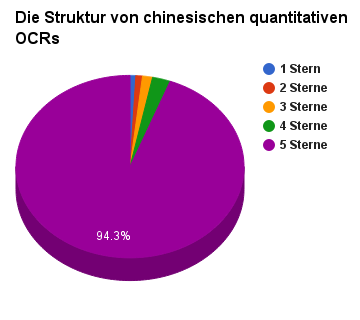
\includegraphics[width=0.5\textwidth]{empirische_ergebnisse/struktur_cn_quantitativ_allgemein}}    
    {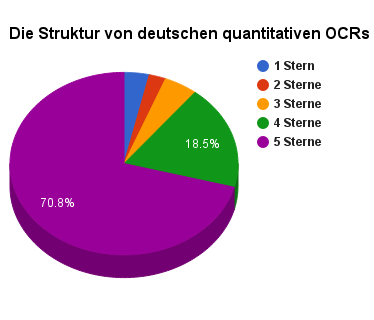
\includegraphics[width=0.5\textwidth]{empirische_ergebnisse/struktur_de_quantitativ_allgemein}}   
    \caption[Die Struktur von den chinesischen und deutschen quantitativen OCRs in Allgemeinen]{Die Struktur von den chinesischen und deutschen quantitativen \ac{OCRs} in Allgemeinen (Quelle: Eigene Darstellung)}
    \label{fig:struktur_allgemein}
\end{figure}

\begin{figure}[htb]
    \minipage{0.5\textwidth}
    \includegraphics[page=4,width=\linewidth]{empirische_ergebnisse/gesammt_cn_sentiment.pdf}
    \endminipage\hfill
    \minipage{0.5\textwidth}
    \includegraphics[page=4,width=\linewidth]{empirische_ergebnisse/gesammt_de_sentiment.pdf}
    \endminipage 
    \caption[Die Verteilungen der chinesischen und deutschen Valenzen von den qualitativen OCRs in Allgemeinen]{Die Verteilungen der chinesischen und deutschen Valenzen von den qualitativen \ac{OCRs} in Allgemeinen (Die blauen Linien sind die entsprechende Normalverteilung.) (Quelle: Eigene Darstellung)}
    \label{fig:valenz_allgemein}
\end{figure}

In den Abbildungen \ref{fig:struktur_allgemein} und \ref{fig:valenz_allgemein} kann man feststellen, dass die chinesischen Kunden viel mehr gerne ``fünf Sterne'' als die quantitativen Bewertungen für die Produkte geben, aber gleichzeitig drücken sie ihre Gefühlen zentralisierter und dichter über die Produkte aus. Die Deutschen geben nicht so viele ``fünf Sterne'' aus, und sie drücken vielfähiger und individueller von ihren Gefühlen durch die qualitativen \ac{OCRs} aus. Auch aus dieser Abbildung kann man die Nullhypothese in Abschnitt \ref{sec:h0} ablehen.

\begin{table}[htb]
\centering
%\resizebox{\textwidth}{!}{%
\begin{tabular}{|c|c|c|}
\hline
            & \begin{tabular}[c]{@{}c@{}}Valenz von \\ quantitativen \ac{OCRs}\end{tabular} & \begin{tabular}[c]{@{}c@{}}Valenz von \\ qualitativen \ac{OCRs}\end{tabular} \\ \hline
China       & 4,884933                                                                 & 0,2525381                                                                            \\ \hline
Deutschland & 4,505952                                                                 & 0,6701946                                                                            \\ \hline
\end{tabular}
%}
\caption[Die Valenzen von den chinesischen und deutschen OCRs an der quantitativen und qualitativen Seite]{Die Valenzen und von den chinesischen und deutschen \ac{OCRs} an der quantitativen und qualitativen Seite (Quelle: Eigene Darstellung)}
\label{tab:valenzen_allgemein}
\end{table}

In der Tabelle \ref{tab:valenzen_allgemein} sieht man schon, dass die deutschen qualitativen Bewertungen viel positiver als die Chinesischen sind, obwohl die Deutschen normallerweise kleinere Sterne als die Chinesen gegeben haben. Durch diese Ergebnisse stimmt die Hypothese \ref{hyp:2} nur an der qualitativen Seite in Allgemeinen. 

%%=======================================
\section{Hypothese 3}
%%=======================================
Bei der Hypothese \ref{hyp:3} gibt es einen theoretischen Widerspruch. Einerseits erzeugt große Machtdistanz Ungleichheit und damit große Varianz von Valenzen der \ac{OCRs} nach \citet{hofstede2013interkulturelle}. Andererseits meinen \citeauthor{Luo2014} dass die \ac{OCRs} konsistenter beim Kollektivismus sein werden. Deswegen sollte die Varianz von Valenzen der chinesischen \ac{OCRs} kleiner sein. In diesem Abschnitt wird dieser Konflikt bei jedem Artikel und in Allgemeinen getestet, um eine dominierende Dimension herauszufinden.
%%=======================================
\subsection{Hypothese 3 bei jedem Artikel} \label{sec:h3_jeweils}
%%=======================================
Die Varianz beschreibt wie stark die Meinungen und Gefühlen von Menschen in den \ac{OCRs} schwanken. Verschiedenen Artikeln, obwohl in gleicher Kategorie oder bei gleicher Marke, sind für die Menschen unterschiedlich, weil sie vielleicht unterschiedlich Qualität haben. Deshalb ist es besser, getrennt beim jeden Artikel zu analysieren, als in Kategorien oder Marken.

Wie es am Ende des Abschnitts \ref{sec:untersuchungsobjekt} schrieben wird, sind die zwei T-Shirts jeweils von Nike und Puma, und die beiden Hosen werden eine männliche und eine weibliche von Adidas produziert. Deshalb sie werden in dieser Arbeit nach Marken und Geschlecht genannt. 

Um die Heterogenität der Varianzen besser zu bestimmen, wird der Levene-Test hier durchgeführt. Der Levene-Test bezeichnet in der Statistik einen Signifikanztest, der auf Gleichheit der Varianzen (Homoskedastizität) von zwei oder mehr Grundgesamtheiten (Gruppen) prüft. Der Levene-Test prüft die Nullhypothese darauf, dass alle Gruppenvarianzen gleich sind. \citep{levene1960robust} Wenn sich der Signifikanzwert des Tests unter einem zuvor bestimmten Niveau befindet, sind die Heterogenität der Varianzen der Stichproben signifikant und die Nullhypothese der Varianzgleichheit kann abgelehnt werden. \citep{martens2003statistische}
\begin{table}[htb]
\centering
\begin{tabular}{|c|c|c|}
\hline
\multirow{2}{*}{p-Wert}                                   & \multicolumn{2}{c|}{Varianzheterogenität in deutschen und chinesischen} \\ \cline{2-3} 
                                                          & quantitative OCRs                   & qualitative OCRs                  \\ \hline
\begin{tabular}[c]{@{}c@{}}Adidas\\ männlich\end{tabular} & 0,04948                             & 0,0006272                         \\ \hline
\begin{tabular}[c]{@{}c@{}}Adidas\\ weiblich\end{tabular} & 0,03005                             & 0,0001619                         \\ \hline
Nike                                                      & $9,003\times 10^{-06}$                           & $2,511 \times 10^{-08}$                         \\ \hline
Puma                                                      & \textbf{0,22}                       & 0,0002532                         \\ \hline
\end{tabular}
\caption[Die Ergebnisse des Levene-Tests beim jeden Artikel]{Die Ergebnisse des Levene-Tests beim jeden Artikel (Signifikanzniveau $\alpha = 0,05$) (Quelle: Eigene Darstellung)}
\label{tab:levene_jeweils}
\end{table}

Wie in der Tabelle ersichtlich, sind die p-Werte fast alle kleiner als das Signifikanzniveau $\alpha$, außer den zwischen quantitativen \ac{OCRs} von Puma. Der Wert 0,22 ist die einzelne Ausnahme. Für diese Außerordentlichkeit kann man nicht die Nullhypothese des Levene-Tests ablehnen, aber für die Anderen zeigt der Levene-Test, dass die Varianzen ungleich sind. Das heißt, dass es die Varianzheterogenität in deutschen und chinesischen quantitativen und qualitativen \ac{OCRs} bei der Mehrheit der Produkten gibt. 

\begin{table}[htb]
\centering
\begin{tabular}{|c|c|c|c|c|}
\hline
\multirow{2}{*}{Artikel}                                  & \multicolumn{2}{c|}{\begin{tabular}[c]{@{}c@{}}Varianz \\ von quantitativen OCRs\end{tabular}} & \multicolumn{2}{c|}{\begin{tabular}[c]{@{}c@{}}Varianz \\ von qualitativen OCRs\end{tabular}} \\ \cline{2-5} 
                                                          & China                                             & Deutschland                                           & China                                            & Deutschland                                           \\ \hline
\begin{tabular}[c]{@{}c@{}}Adidas\\ männlich\end{tabular} & 0,6666667                                            & 1,552525                                                & 0,0950417                                           & 0,4937723                                                \\ \hline
\begin{tabular}[c]{@{}c@{}}Adidas\\ weiblich\end{tabular} & 0,5356501                                            & 1,25                                                & 0,134694                                           & 0,3634815                                                \\ \hline
Nike                                                      & 0,1920619                                            & 0,8102564                                                & 0,1421846                                           & 0,4902091                                                \\ \hline
Puma                                                      & 0,498598                                            & 0,323049                                                & 0,1991728                                           & 0,3641573                                                \\ \hline
\end{tabular}
\caption[Die Varianzen der quantitativen und qualitativen OCRs von jedem Artikel]{Die Varianzen der quantitativen und qualitativen \ac{OCRs} von jedem Artikel (Quelle: Eigene Darstellung)}
\label{tab:sd_jeweils}
\end{table}
Tabelle \ref{tab:sd_jeweils} zeigt die Varianzen der quantitativen und qualitativen \ac{OCRs} von jedem Artikel. Wie sich bereits aus der Tabelle ersehen lässt, ist jede Varianz von chinesischen qualitativen \ac{OCRs} über eigenes Untersuchungsobjekt kleiner als die von deutschen, obwohl die Varianzen von deutschen quantitativen \ac{OCRs} nicht alle größer als die von chinesischen sind. Das heißt: Die Grade der Verschiedenheiten von deutschen und chinesischen quantitativen \ac{OCRs} sind unbedingt, aber die Valenzen von deutschen qualitativen \ac{OCRs} schwanken stärker als die von chinesischen. Anders gesagt, es gibt mehrere Ungleichheiten in den Gefühlen der deutschen Kunden als von der chinesischen Kunden. Dies erklärt auch, dass die Gefühlen der chinesischen Kunden über das Produkt viel dichter in der Nähe des Mittelwertes als die Gefühlen von Deutschen sind.

Aus Tabelle \ref{tab:sd_jeweils} kann man auch anders erfassen. Weil die beiden Produkte von Adidas Hose sind, sind die Varianzen von deutschen quantitativen \ac{OCRs} aller größer als die von chinesischen. In Kategorie T-Shirt ist die Situation anders. Die Artikeln von Nike und Puma sind T-Shirt, aber die Varianzen bleiben heterogen. Im Bereich ``Varianz von quantitativen \ac{OCRs}'' sind die deutschen Valenzen von Produkten aus Adidas und Nike größer als die chinesischen, aber die Valenz von Puma ist eine Ausnahme, die schon in Tabelle \ref{tab:levene_jeweils} kennzeichnet wird. Außer der Ausnahme, sind die Varianzen von chinesischen \ac{OCRs} kleiner als die deutschen. Die Hypothese \ref{hyp:3} wird bei jedem Artikel nur teilweise gestützt. 
%%=======================================
\subsection{Hypothese 3 in Allgemeinen}
%%=======================================
In diesem Abschnitt wird die Varianzen in einer allgemeinen Hinsicht verglichen. Damit wird es besser erfasst, wie die deutschen und chinesischen Kunden in Allgemeinen verhalten haben. Die Unterschiede zwischen Marken oder Kategorien werden ausgeglichen.

\begin{table}[htb]
\centering
\begin{tabular}{|l|l|l|}
\hline
allgemein & quantitative \ac{OCRs} & qualitative \ac{OCRs}  \\ \hline
p-Wert    & $< 2,2 \times 10^{-16}$ & $< 2,2 \times 10^{-16}$  \\ \hline
\end{tabular}
\caption[Die Ergebnisse von Levene-Test in Allgemeinen]{Die Ergebnisse von Levene-Test in Allgemeinen (Signifikanzwert $\alpha = 0,05$) (Quelle: Eigene Darstellung)}
\label{tab:levene_allgemein}
\end{table}

In dieser Tabelle kann man durch betrachten der p-Werte von Levene-Test schließen, dass sie alle kleiner als den Signifikanzwert $\alpha$ sind. Die Tabelle \ref{tab:levene_allgemein} stützt die Ergebnisse von Tabelle \ref{tab:varianz_allgemein}. Durch den Levene-Test sind die Varianzen zwischen den \ac{OCRs} von China und Deutschland heterogen.

\begin{table}[htb]
\centering
\begin{tabular}{|c|c|c|}
\hline
Varianz                & China     & Deutschland \\ \hline
von quantitativen \ac{OCRs} & 0,2855922 & 0,92212     \\ \hline
von qualitativen \ac{OCRs}  & 0,1518924 & 0,4284648   \\ \hline
\end{tabular}
\caption[Die Varianzen von den chinesischen und deutschen OCRs]{Die Varianzen von den chinesischen und deutschen \ac{OCRs} (Quelle: Eigene Darstellung)}
\label{tab:varianz_allgemein}
\end{table}

Tabelle \ref{tab:varianz_allgemein} zeigt die Ergebnisse. Dieser Tabelle kann man auch entnehmen, dass die deutschen Varianzen größer als die chinesischen sind. Die Meinungen sowie die Gefühlen der chinesischen Kunden liegen meistens in der Mittel während die Meinungen und Gefühlen der deutschen Kunden schwanken hin und her. Die Varianzen von qualitativen \ac{OCRs} sind kleiner als die von quantitativen \ac{OCRs} für die Kunden aus beiden Ländern. Das bedeutet, dass die quantitativen \ac{OCRs} viel zufallsbedingter als die qualitativen \ac{OCRs}. Mit anderen Worten sind die quantitativen \ac{OCRs} nicht so glaubwürdig, aber die Gefühlen von Kunden werden nicht so viel von externer Faktoren beeinflusst. Durch diesen Ergebnisse wird Hypothese \ref{hyp:3} in allgemeiner Weise gestützt.
%%=======================================
\section{Hypothese 4} \label{sec:h4}
%%=======================================
Obwohl es viele Forschungen über die \acl{OCRs} schon gab, gibt es noch niemand anhand, wer über den Zusammenhang zwischen den quantitativen und qualitativen \ac{OCRs} studiert. Man dachte, dass es bestimmten Zusammenhang dazwischen gibt, aber ist es wirklich so? Wenn ja, ist der Zusammenhang linear oder unlinear? Gibt es kulturelle Einflüsse auf den Zusammenhang? Diese Fragen haben noch nie geantwortet geworden. In diesem Abschnitt werden die Antworten in Möglichweise ausgefunden.
%%=======================================
\subsection{Hypothese 4 bei jedem Artikel} \label{sec:h4_jeweils}
%%=======================================
Wie bereits erwähnt weiß man noch nichts über den Zusammenhang zwischen den quantitativen und qualitativen \ac{OCRs}. Die erste Aufgabe von Hypothese \ref{hyp:4} ist, zu bestimmen, ob der Zusammenhang tatsächlich existiert. Deshalb wird der Test von jedem Artikel erst durchgeführt. 

Als ersten Schritt ist es anzunehmen, dass der Zusammenhang linear ist. Von daher wird erst der Korrelationstest von Pearson zwischen den Valenzen von quantitativen und qualitativen \ac{OCRs} durchgeführt. Der Test beginnt mit einer Nullhypothese, die setzt voraus, dass es keinen lineare Zusammenhang zwischen den Valenzen der quantitativen und qualitativen \ac{OCRs} gibt. Ist der p-Wert kleiner als das Signifikanzniveau $\alpha$, wird die Nullhypothese abgelehnt, also: Es gibt linearen Zusammenhang dazwischen. \citep{pearson1895note}

\begin{table}[h]
\centering
\begin{tabular}{|c|c|c|}
\hline
p-Wert                                                    & China     & Deutschland \\ \hline
\begin{tabular}[c]{@{}c@{}}Adidas\\ männlich\end{tabular} & \textbf{0,5251}    & 0,001808    \\ \hline
\begin{tabular}[c]{@{}c@{}}Adidas\\ weiblich\end{tabular} & 0,0002521 & \textbf{0,07921}     \\ \hline
Nike                                                      & $2,911 \times 10^{-05}$ & 0,02091     \\ \hline
Puma                                                      & $5,148 \times 10^{-07}$ & \textbf{0,9997}      \\ \hline
\end{tabular}
\caption[Die Ergebnisse von Pearsons Korrelationstest bei jedem Artikel]{Die Ergebnisse von Pearsons Korrelationstest bei jedem Artikel (Signifikanzniveau $\alpha = 0,05$) (Quelle: Eigene Darstellung)}
\label{tab:pearson_test_jeweils}
\end{table}

Die Ergebnistabelle \ref{tab:pearson_test_jeweils} gibt die p-Werte von jedem Artikel an. Wie sich bereits aus der Tabelle ersehen lässt, sind die p-Werte nicht alle kleiner als das Signifikanzniveau $\alpha$. Für die chinesischen \ac{OCRs}, kann man nicht die Nullhypothese bei der männlichen Hose aus Adidas ablehnen, aber bei den Anderen wird die Nullhypothese abgelehnt. An der deutschen Seite, ist die Situation anders. Bei der weiblichen Hose aus Adidas und dem T-Shirt aus Puma, wird die Nullhypothese nicht ablehnt, während man bei den anderen zwei Artikeln die Nullhypothese ablehnen kann.

Dies bedeutet, dass es linearen Zusammenhang zwischen den chinesischen Valenzen von quantitativen und qualitativen \ac{OCRs} gibt, außer der, deren \ac{OCRs} für männlichen Hose aus Adidas sind. Für die Valenzen von den deutschen \ac{OCRs}, existiert der lineare Zusammenhang bei der männlichen Hose aus Adidas und dem T-Shirt aus Nike. 

Bei den Artikeln, deren p-Werte größer als 0,05 sind, kann man nicht direkt sagen, dass es keinen linearen Zusammenhang dazwischen gibt. Ebenso, stellt ein kleiner p-Wert nicht großen Zusammenhang dar. Die tatsächlichen Ergebnisse von Pearson's Korrelationskoeffizient ${\rho}_p$ werden durch Tabelle \ref{tab:pearson_korrelation_jeweils} dargestellt.

\begin{table}[h]
\centering
\begin{tabular}{|c|c|c|}
\hline
${\rho}_p$                                                         & China      & Deutschland \\ \hline
\begin{tabular}[c]{@{}c@{}}Adidas\\ männlich\end{tabular} & 0,1333677  & 0,4523909   \\ \hline
\begin{tabular}[c]{@{}c@{}}Adidas\\ weiblich\end{tabular} & 0,2337115  & 0,3576531   \\ \hline
Nike                                                      & 0,09517316 & 0,3640926   \\ \hline
Puma                                                      & 0,2269939  & $-5,7147 \times 10^{-05}$ \\ \hline
\end{tabular}
\caption[Die Pearsons Korrelationskoeffizienten ${\rho}_p$ zwischen den chinesischen und deutschen Valenzen der quantitativen und qualitativen OCRs]{Die Pearsons Korrelationskoeffizienten ${\rho}_p$ zwischen den chinesischen und deutschen Valenzen der quantitativen und qualitativen \ac{OCRs} (Quelle: Eigene Darstellung)}
\label{tab:pearson_korrelation_jeweils}
\end{table}

Aus der Tabelle ist ersichtlich, dass die Korrelationskoeffizienten ${\rho}_p$ fast alle positiv sind, außerdem Puma Deutschland. Der Korrelationskoeffizient von den Valenzen der deutschen \ac{OCRs} ist eine Ausnahme, wie es im Abschnitt \ref{sec:h3_jeweils} schon einmal passiert ist. Diese Ausnahme zeigt auch, dass die deutschen quantitativen \ac{OCRs} von Puma kaum Zusammenhang mit den qualitativen \ac{OCRs} haben. Wenn man außer der Außordentlichkeit sieht, kann man erfassen, dass die anderen nicht nur positiv sind, die deutschen Korrelationskoeffizienten sind auch größer als die chinesischen.

Diese Ergebnisse bedeuten, dass der lineare Zusammenhang zwischen den meisten quantitativen und qualitativen \ac{OCRs} existiert. Und sie sind positiv abhängig. In meisten Situationen sind die linearen Zusammenhangen von chinesischen \ac{OCRs} kleiner als die von deutschen \ac{OCRs}. Auf dieser Weise wird Hypothese \ref{hyp:4} teilweise gestützt.

Aber vielleicht ist der Zusammenhang nicht linear. Um den tatsächlichen Zusammenhang zwischen den quantitativen und qualitativen \ac{OCRs} auszufinden, wird der Spearmans Rangkorrelation-Test durchgeführt.

\begin{table}[h]
\centering
\begin{tabular}{|c|c|c|}
\hline
p-Wert                                                    & China           & Deutschland      \\ \hline
\begin{tabular}[c]{@{}c@{}}Adidas\\ männlich\end{tabular} & \textbf{0,9555} & 0,0002549        \\ \hline
\begin{tabular}[c]{@{}c@{}}Adidas\\ weiblich\end{tabular} & 0,001942        & \textbf{0,06097} \\ \hline
Nike                                                      & $4,813 \times 10^{-07}$       & 0,002007         \\ \hline
Puma                                                      & $1,173 \times 10^{-09}$       & \textbf{0,5814}  \\ \hline
\end{tabular}
\caption[Die Ergebnisse von Spearmans Rangkorrelationstest bei jedem Artikel]{Die Ergebnisse von Spearmans Rangkorrelationstest bei jedem Artikel (Signifikanzniveau $\alpha = 0,05$) (Quelle: Eigene Darstellung)}
\label{tab:spearman_test_jeweils}
\end{table}

Der Spearmans Rangkorrelationskoeffizient ist ein parameterfreies Maß für Korrelationen. Das bedeutet, dass er misst, wie gut eine beliebige monotone Funktion den Zusammenhang zwischen zwei Variablen (In dieser Arbeit sind die quantitativen und qualitativen Valenzen) beschreiben kann, ohne irgendwelche die Wahrscheinlichkeitsverteilung der Variablen anzunehmen. \citep{meyer1969spearmans}

Die Ergebnisse von Spearmans Rangkorrelationstest sind nicht anders wie die Ergebnisse von Pearsons Korrelationstest. Der Tabelle \ref{tab:spearman_test_jeweils} ist zu entnehmen, dass die drei p-Werte, die in gleichen Positionen in Tabelle \ref{tab:pearson_test_jeweils} sind, größer als das Signifikanzniveau 0,05 sind. Und Tabelle \ref{tab:spearman_korrelation_jeweils} zeigt die Spearmans Rangkorrelationskoeffizienten $rho$ bei jedem Artikel.

\begin{table}[h]
\centering
\begin{tabular}{|c|c|c|}
\hline
$rho$                                                       & China      & Deutschland          \\ \hline
\begin{tabular}[c]{@{}c@{}}Adidas\\ männlich\end{tabular} & 0,01176353 & 0,5195352            \\ \hline
\begin{tabular}[c]{@{}c@{}}Adidas\\ weiblich\end{tabular} & 0,1986592  & 0,3799971            \\ \hline
Nike                                                      & 0,1144833  & 0,473936             \\ \hline
Puma                                                      & 0,2733825  & \textbf{-0,07389644} \\ \hline
\end{tabular}
\caption[Die Spearmans Rangkorrelationskoeffizienten $rho$ zwischen den chinesischen und deutschen Valenzen der quantitativen und qualitativen OCRs]{Die Spearmans Rangkorrelationskoeffizienten $rho$ zwischen den chinesischen und deutschen Valenzen der quantitativen und qualitativen \ac{OCRs} (Quelle: Eigene Darstellung)}
\label{tab:spearman_korrelation_jeweils}
\end{table}

Die Ergebnisse in Tabelle \ref{tab:spearman_korrelation_jeweils} sind sehr ähnlich wie sie in Tabelle \ref{tab:pearson_korrelation_jeweils}. Außer der Ausnahme von Puma Deutschland, sind die deutschen Spearmans Rangkorrelationskoeffizienten $rho$ größer als die chinesischen, und die alle $rho$ sind größer als 0. Diese Ergebnisse zeigen, dass es einen positiven Zusammenhang zwischen den meisten quantitativen und qualitativen \ac{OCRs} in beiden Ländern gibt. Und der Zusammenhang bei den deutschen Kunden ist mehrheitlich größer als der bei den Chinesen. Dadurch wird die Hypothese \ref{hyp:4} in den meisten Fällen gestützt.
%%=======================================
\subsection{Hypothese 4 in Allgemeinen}
%%=======================================
Abschnitt \ref{sec:h4_jeweils} gibt schon die Übersicht über jeden Artikel an, und in diesem Abschnitt kann man eine allgemeine Hinsicht über den Zusammenhang haben. Die Unterschiede von den jeweiligen Artikeln werden ausgeglichen, um besser das Kennzeichen von China oder Deutschland zu verstehen. 

Abbildung \ref{fig:valenzen_de_cn_allgemein} zeigt die Verteilung der quantitativen und qualitativen \ac{OCRs} von China und Deutschland. Jeder Farbblock zeigt eine qualitative Valenz. Der dunkelrote Block repräsentiert Valenz 0, und der Pinke ist Valenz 0,3716, die in dem Lexion ``gut'' besteht. Der Abbildung ist zu entnehmen, dass viele chinesischen Kunden nichts über ihre Attitude oder nur ein ``gut'' geschrieben, obwohl sie schon fünf Sterne gegeben haben. Und die deutschen Kunden geben ihre qualitativen Bewertung viel individueller als die Chinesischen. Anders gesagt, die Korrelation zwischen den quantitativen und qualitativen \ac{OCRs} sind in China und Deutschland unterschiedlich. Um diese Unterschiede zu erkennen, werden der Pearsons Korrelationstest und der Spearmans Rangkorrelationstest durchgeführt.

\begin{table}[h]
\centering
\begin{tabular}{|c|c|c|}
\hline
Pearson & China     & Deutschland \\ \hline
p-Wert  & $2,665 \times 10^{-15}$ & $1,629 \times 10^{-05}$   \\ \hline
${\rho}_p$     & 0,1522703 & 0,3258736   \\ \hline
\end{tabular}
\caption[Die Ergebnisse von Pearsons Korrelationstest zwischen quantitativen und qualitativen OCRs in China und Deutschland in Allgemeinen]{Die Ergebnisse von Pearsons Korrelationstest zwischen quantitativen und qualitativen \ac{OCRs} in China und Deutschland in Allgemeinen (Signifikanzniveau $\alpha = 0,05$) (Quelle: Eigene Darstellung)}
\label{tab:pearson_allgemein}
\end{table}

Tabelle \ref{tab:pearson_allgemein} zeigt die Ergebnisse im Signifikanzniveau $\alpha = 0,05$ mit der Nullhypothese, die ist, dass es keinen linearen Zusammenhang gibt. Der Tabelle ist zu entnehmen, dass die alle p-Werte kleiner als das Signifikanzniveau sind. Das bedeutet, dass die Nullhypothese abgelehnt wird. Also, es gibt linearen Zusammenhang zwischen quantitativen und qualitativen \ac{OCRs} in den beiden Ländern. ${\rho}_p$ sind in beiden Ländern positiv. Das heißt, dass der Zusammenhang in Allgemeinen positiv ist. Aber die Korrelationskoeffizienten von den beiden Ländern sind klein, trotz der von Deutschland größer ist. Das ist die Ergebnisse von linearem Zusammenhang. Die Tabelle \ref{tab:spearman_allgemein} zeigt die Ergebnisse, wenn der Zusammenhang nicht linear ist.

\begin{table}[h]
\centering
\begin{tabular}{|c|c|c|}
\hline
Spearman & China             & Deutschland \\ \hline
p-Wert   & $< 2,2 \times 10^{-16}$ & $5,967 \times 10^{-05}$   \\ \hline
$rho$      & 0,1632395         & 0,3045776   \\ \hline
\end{tabular}
\caption[Die Ergebnisse von Spearmans Rangkorrelationstest zwischen quantitativen und qualitativen OCRs in China und Deutschland in Allgemeinen]{Die Ergebnisse von Spearmans Rangkorrelationstest zwischen quantitativen und qualitativen \ac{OCRs} in China und Deutschland in Allgemeinen (Signifikanzniveau $\alpha = 0,05$) (Quelle: Eigene Darstellung)}
\label{tab:spearman_allgemein}
\end{table}

Die Ergebnisse in Tabelle \ref{tab:spearman_allgemein} sind nichts anders als die in Tabelle \ref{tab:pearson_allgemein}. Dadurch wird bestimmt: obwohl die quantitativen und qualitativen \ac{OCRs} einen positiven Zusammenhang dazwischen haben, aber der Zusammenhang ist nicht stark. Anders gesagt, es ist nicht genug, wenn man nur über die quantitativen \ac{OCRs} studieren, weil der schriftlicher Teil mehr das wirkliche Gefühl von Kunden über das Produkt ausdrücken kann. 

Diese Ähnlichkeit zeigt auch, dass dieser Zusammenhang linear sein könnte, obwohl er nicht so stark ist. Der Unterschied zwischen den Korrelationskoeffizienten oder Rangkorrelationskoeffizienten bedeutet auch, dass die kulturellen Einflüsse unterschiedlich auf den quantitativen und qualitativen \ac{OCRs} sind.

In allgemeiner Hinsicht ist der Zusammenhang zwischen den deutschen quantitativen und qualitativen \ac{OCRs} stärker. Besonders bei China, sind die meistens quantitativen Bewertung als fünf Sterne (siehe Abbildung \ref{fig:struktur_allgemein}), aber der Korrelationskoeffizient zwischen quantitativen Bewertung und schriftlichen Meinung von Kunden ist kleiner als 0,2. Das zeigt dass die Sterne und die Polarität nicht großen Zusammenhang haben, obwohl sie von einander positiv abhängig sind. Anders gesagt, die quantitative Bewertungen (besonders von chinesischen Kunden) sind nicht so glaubwürdig, wie viele Wirtschaftler geglaubt haben. Vergleich mit chinesischen Bewertungen, sind die deutschen quantitativen \ac{OCRs} glaubwürdiger, weil der Rangkorrelationskoeffizient dazwischen größer ist. Zusammenfassend wird die Hypothese \ref{hyp:4} in allgemeiner Weise gestützt.

\begin{figure}[htb]
    \minipage{\textwidth}
    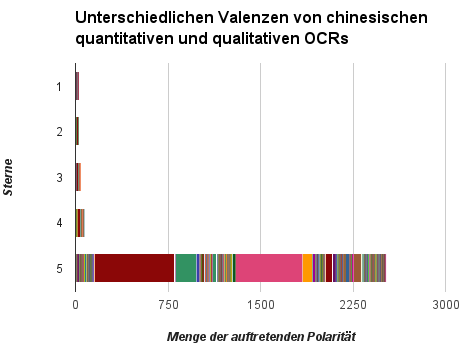
\includegraphics[width=\linewidth]{empirische_ergebnisse/valenzen_cn_allgemein}
    \endminipage\hfill
    \minipage{\textwidth}
    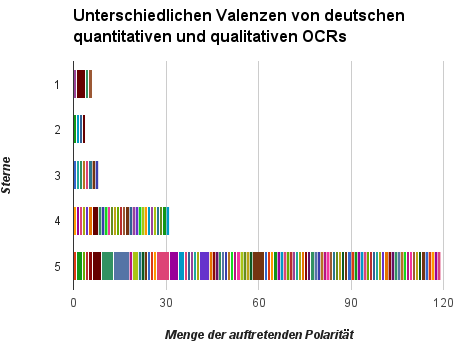
\includegraphics[width=\linewidth]{empirische_ergebnisse/valenzen_de_allgemein}
    \endminipage 
    \caption[Die chinesischen und deutschen Valenzen von den quantitativen und qualitativen OCRs in Allgemeinen]{Die chinesischen und deutschen Valenzen von den quantitativen und qualitativen \ac{OCRs} in Allgemeinen (Quelle: Eigene Darstellung)}
    \label{fig:valenzen_de_cn_allgemein}
\end{figure}


